Avec cette seconde méthode nous allons résoudre l'équation de Poisson à l'aide de la transformée de Fourier. Avant de formuler la résolution de ce problème. Rappelons la définition des opérateurs dont nous aurons besoin dans la suite. \cite{Fourier}
\subsubsection{Rappel et définitions des opérateurs}
\paragraph{Transformée de Fourier (discrète)}
Soit F une fonction, sa transformée de Fourier peut s'écrire de la façon suivante : 
\begin{equation}
\begin{aligned}
\widehat{F}(x,y) = \sum_{k = 0}^{M-1} \sum_{l = 0}^{N-1} F(k,l) e^{-2\pi i\left(\frac{k\times x}{M}+\frac{l\times y}{N}\right)}
\end{aligned}
\end{equation}
Enfin, afin de retrouver la fonction initiale nous aurons besoin de la transformée de Fourier inverse : 
\begin{equation}
\begin{aligned}
F(k,l) = \frac{1}{MN} \sum_{x = 0}^{M-1} \sum_{y = 0}^{N-1} \hat{F}(x,y) e^{2\pi i \left(\frac{xk}{M}+\frac{yl}{N}\right)}
\end{aligned}
\end{equation}
\paragraph{Gradient}
Pour résoudre le problème nous avons besoin de calculer les Laplaciens des images. Nous nous placerons dans le domaine de Fourier, il est donc nécessaire de calculer la transformée de Fourier du Laplacien d'une fonction, et donc le gradient de celle-ci. 
F est toujours la fonction que nous souhaitons étudier. 
\begin{equation}
\begin{aligned}
\widehat{\nabla (F)}=
\begin{pmatrix}
\widehat{\frac{\partial F}{\partial k}}\\
\widehat{\frac{\partial F}{\partial l}}
\end{pmatrix}
\end{aligned}
\end{equation}
En dérivant l'expression ci-dessus par rapport à la première variable : 
\begin{equation}
\begin{aligned}
\frac{\partial F}{\partial k} &= \frac{1}{MN}\sum_{x = 0}^{M-1} \sum_{y = 0}^{N-1} \widehat{F}(x,y) e^{2\pi i\left(\frac{k\times x}{M}+\frac{l\times y}{N}\right)}\left(\frac{2\pi i x}{M}\right)\\
& = \left(\frac{2\pi i x}{M}\right)F(k,l)\\
\widehat{\frac{\partial F}{\partial k}} &= \left(\frac{2\pi i x}{M}\right)\widehat{F(k,l)}
\end{aligned}
\end{equation}
Le calcul est similaire pour $\widehat{\frac{\partial F}{\partial l}}$.\\
On a donc : 
\begin{equation}
\begin{aligned}
\widehat{\frac{\partial F}{\partial k}} = \left(\frac{2\pi i}{M}x\right) \widehat{F}\\
\widehat{\frac{\partial F}{\partial l}} = \left(\frac{2\pi i}{N}y\right) \widehat{F}\\
\end{aligned}
\end{equation}

\paragraph{Laplacien}
\begin{equation}
\begin{aligned}
\frac{\partial^2 F}{\partial k ^2} & = \frac{1}{MN} \sum_{x = 0}^{M-1} \sum_{y = 0}^{N-1} \widehat{F}(x,y) e^{2\pi i\left(\frac{k\times x}{M}+\frac{l\times y}{N}\right)}\left(\frac{2\pi i x}{M}\right)^2\\
& = \left(\frac{2\pi i x}{M}\right)^2 F(k,l)\\
\widehat{\frac{\partial^2 F}{\partial k^2}} &= \left(\frac{2\pi i x}{M}\right)^2\widehat{F(k,l)}
\end{aligned}
\end{equation}
On a donc : 
$\widehat{\Delta F} = \widehat{\frac{\partial^2 F}{\partial k^2}}+ \widehat{\frac{\partial^2 F}{\partial l^2}}$.
\begin{equation}
\widehat{\Delta F} = \left(\frac{2\pi i x}{M}\right)^2 \widehat{F}+\left(\frac{2\pi i y}{N}\right)^2 \widehat{F}
\end{equation}

\subsubsection{Résolution avec la méthode Fourier}
La résolution dans le domaine de Fourier nécessite quelques changements. Cette méthode ne fonctionnant que sur un domaine rectangulaire, nous devons donc modifier le domaine $\Omega$.\\
Rappelons que nous voulons résoudre le problème suivant :
\begin{equation}
\left\{
\begin{aligned}
\Delta I(x,y) = \Delta S(x,y) \ si \ (x,y) \in \Omega\\
I(x,y) = T(x,y) \ si \ (x,y) \notin \Omega
\end{aligned}
\right.
\end{equation}

Nous voulions que le laplacien de I à l'intérieur de $\Omega$ corresponde à celui de S. En considérant le nouveau domaine $\Omega_2$ comme étant l'image entière, il faudrait donc que le Laplacien de I soit très proche du laplacien de $T \cup S$. Mais dans ce cas, nous aurions un fort gradient sur $\partial \Omega$, (le  changement d'intensité entre T et S étant fort). Il faut donc reconsidérer le problème précédent. \\
La nouvelle hypothèse que nous pouvons faire est donc la suivante : $\nabla I$ doit être très proche de $\nabla S$ dans $\Omega$ mais aussi très proche de $\nabla T$ dans $\Omega_2 \backslash \Omega$. En notant V : 
\begin{equation}
V = 
\left\{
\begin{aligned}
\nabla S(x,y) \ si \ (x,y) \in \Omega\\
\nabla T(x,y) \ si \ (x,y) \notin \Omega
\end{aligned}
\right.
= \begin{pmatrix}
V_1\\
V_2
\end{pmatrix}
\end{equation}
\begin{figure}[!htb]
   \begin{minipage}{0.5\textwidth}
     \centering
     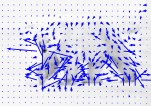
\includegraphics[width = 100pt]{Images/vector_fieldOurs.png}
\caption{Champs de vecteurs de l'image S}
      \end{minipage}\hfill
         \begin{minipage}{0.5\textwidth}
     \centering
     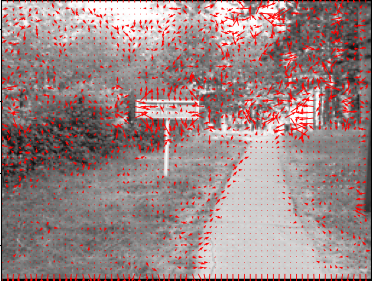
\includegraphics[width = 100pt]{Images/vector_fieldOursT.png}
\caption{Champs de vecteur de l'image T}
      \end{minipage}\hfill
      \end{figure}
Ces images représentent les champs de vecteurs dont le gradient de I devra se rapprocher le plus possible.
      \begin{figure}[!h]
        \begin{minipage}{0.5\textwidth}
     \centering
      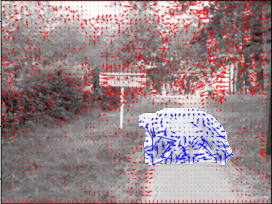
\includegraphics[scale=0.5]{Images/V.png}
      \caption{Nouveau domaine}
      \end{minipage}\hfill
              \begin{minipage}{0.5\textwidth}
     \centering
      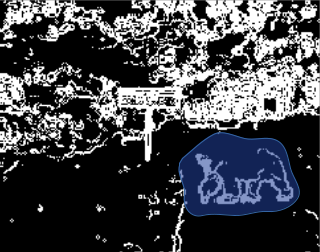
\includegraphics[scale=0.4]{Images/gradient.png}
      \caption{Nouveau domaine}
      \end{minipage}\hfill
      \end{figure}
Nous devons donc résoudre l'équation suivante : 
\begin{center}
$ \Delta I = div(V)$
\end{center}
Afin de pouvoir résoudre cette équation il faut imposer des conditions sur le bord. En appliquant l'effet miroir à l'image correspondant au nouveau domaine, nous obtenons un signal symétrique et il est donc possible d'appliquer la transformée de Fourier pour résoudre le problème.  Les conditions imposées sont donc des conditions de Neumann.

Ainsi en calculant la transformée de Fourier du Laplacien nous obtenons : $\widehat{\Delta I} = \widehat{div(V)}$

\begin{equation}
\begin{aligned}
\left(\frac{2\pi i x}{M}\right)^2 \widehat{I}+\left(\frac{2\pi i y}{N}\right)^2 \widehat{I} & = \left(\frac{2\pi i x}{M}\right) \widehat{V_1}+\left(\frac{2\pi i y}{N}\right) \widehat{V_2}\\
\left(\left(\frac{2\pi i x}{M}\right)^2+\left(\frac{2\pi i y}{N}\right)^2\right) \widehat{I} & = \left(\frac{2\pi i x}{M}\right) \widehat{ V_1}+\left(\frac{2\pi i y}{N}\right) \widehat{V_2}\\
\end{aligned}
\end{equation}
\begin{equation}
\begin{aligned}
\widehat{I} = \frac{\left(\frac{2\pi i x}{M}\right) \widehat{ V_2}+\left(\frac{2\pi i y}{N}\right) \widehat{V_1}}{\left(\left(\frac{2\pi i x}{M}\right)^2+\left(\frac{2\pi i y}{N}\right)^2\right)}
\end{aligned}
\end{equation}
Afin de retrouver I, il suffit d'appliquer la transformée inverse, à l'équation ci-dessus.
Les résultats obtenus avec cette méthode seront présentés dans une prochaine section. 